\chapter{Evaluation}
\section{Presence notifications}
I had three rosters for testing purposes: \code{roster/alice.xml}, \code{roster/bob.xml}, \code{roster/caroll.xml}. Their mutual subscriptions demonstrate the four combinations \code{none}, \code{from}, \code{to}, and \code{both}.
[sub graph??]
The 
The logs show that their consecutive connections produce the correct presence-notification patterns in accordance with their subscriptions to each other.

\section{Roster management}
I have evidence that in the aforementioned connections the clients receive their rosters as expected. The lack of CRUD operations means there is little else to do.

\section{Handshake; connect / disconnect}
I have screenshot and logs collectively showing the following:
\begin{itemize}
  \item Working handshake between Psi and server, plus appropriate \code{feature-not-implemented} response to the non-core features Psi requests
  \item Conversation between Bob and Caroll via the Psi messaging interface and the \code{Client} module respectively
\end{itemize}
Figure~\ref{fig:iq-errors} demonstrates an attempt by Bob to connect to the server using Psi. After a successful handshake, Psi gave an error dialog (not shown) because of the unsupported features, as seen in the server output. For example:

\begin{xml}
<iq xmlns="jabber:client" type="get" id="aacaa" >
  <query xmlns="jabber:iq:private" >
   <storage xmlns="storage:bookmarks"/>
  </query>
</iq>
\end{xml}

is answered with

\begin{xml}
<iq type="error" id="aacaa" >
  <error type="cancel" >
    <feature-not-implemented xmlns="urn:ietf:params:xml:ns:xmpp-stanzas"/>
  </error>
</iq>
\end{xml}

Psi still continued with the protocol and registered Bob as online. When Caroll connected via the \code{Client} module in the OCaml toplevel, the notification ``Caroll is online'' appeared in the top right-hand corner of the screen. Figure~\ref{caroll-msg} shows the result of two messages; Caroll sends hers with \code{caroll#message_t} and Bob sends his using the Psi interface. Entering \code{caroll#spill} in the toplevel showed that both Caroll's initial presence and Bob's message arrived properly.

\begin{figure}
  \centering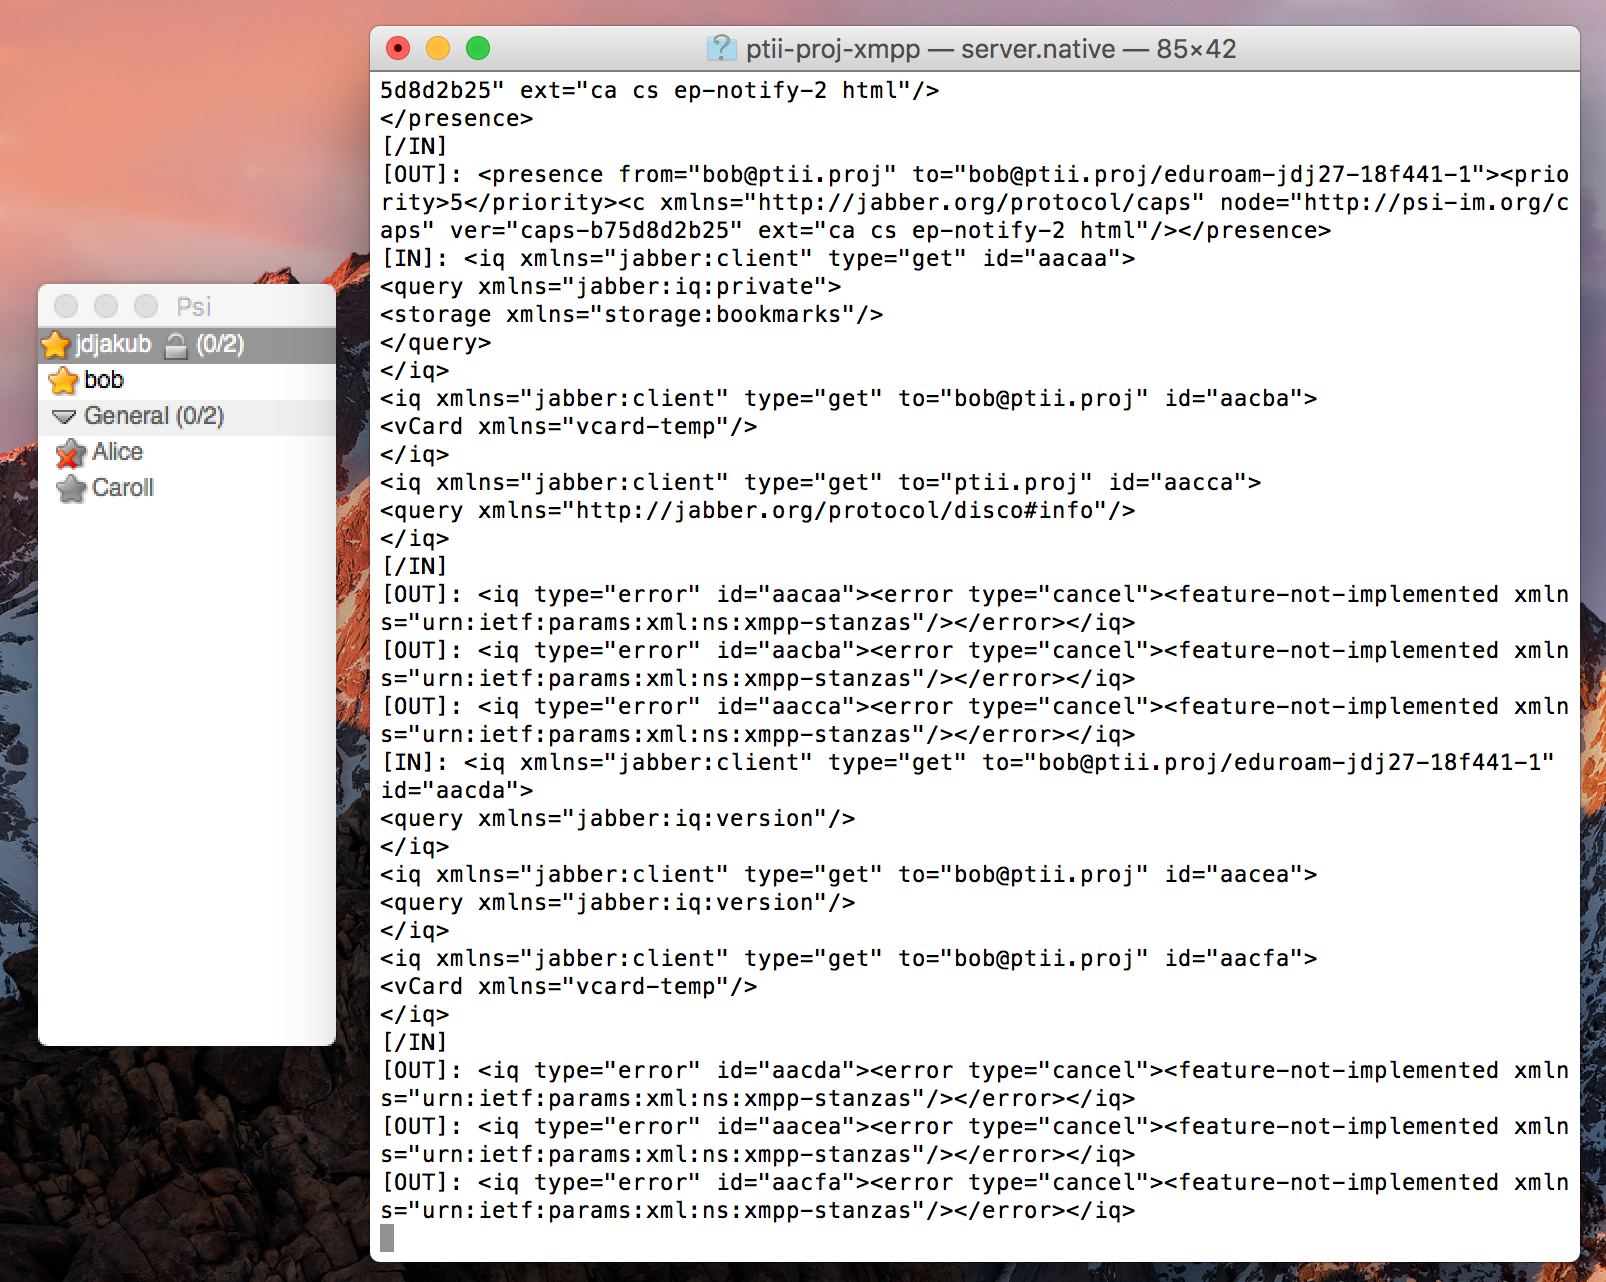
\includegraphics[width=\textwidth]{../transcripts/iq_errors.png}
  \caption{Response to unsupported IQ messages, after which Bob shows as Online in the Psi interface.}
  \label{fig:iq-errors}
\end{figure}

\begin{figure}
  \centering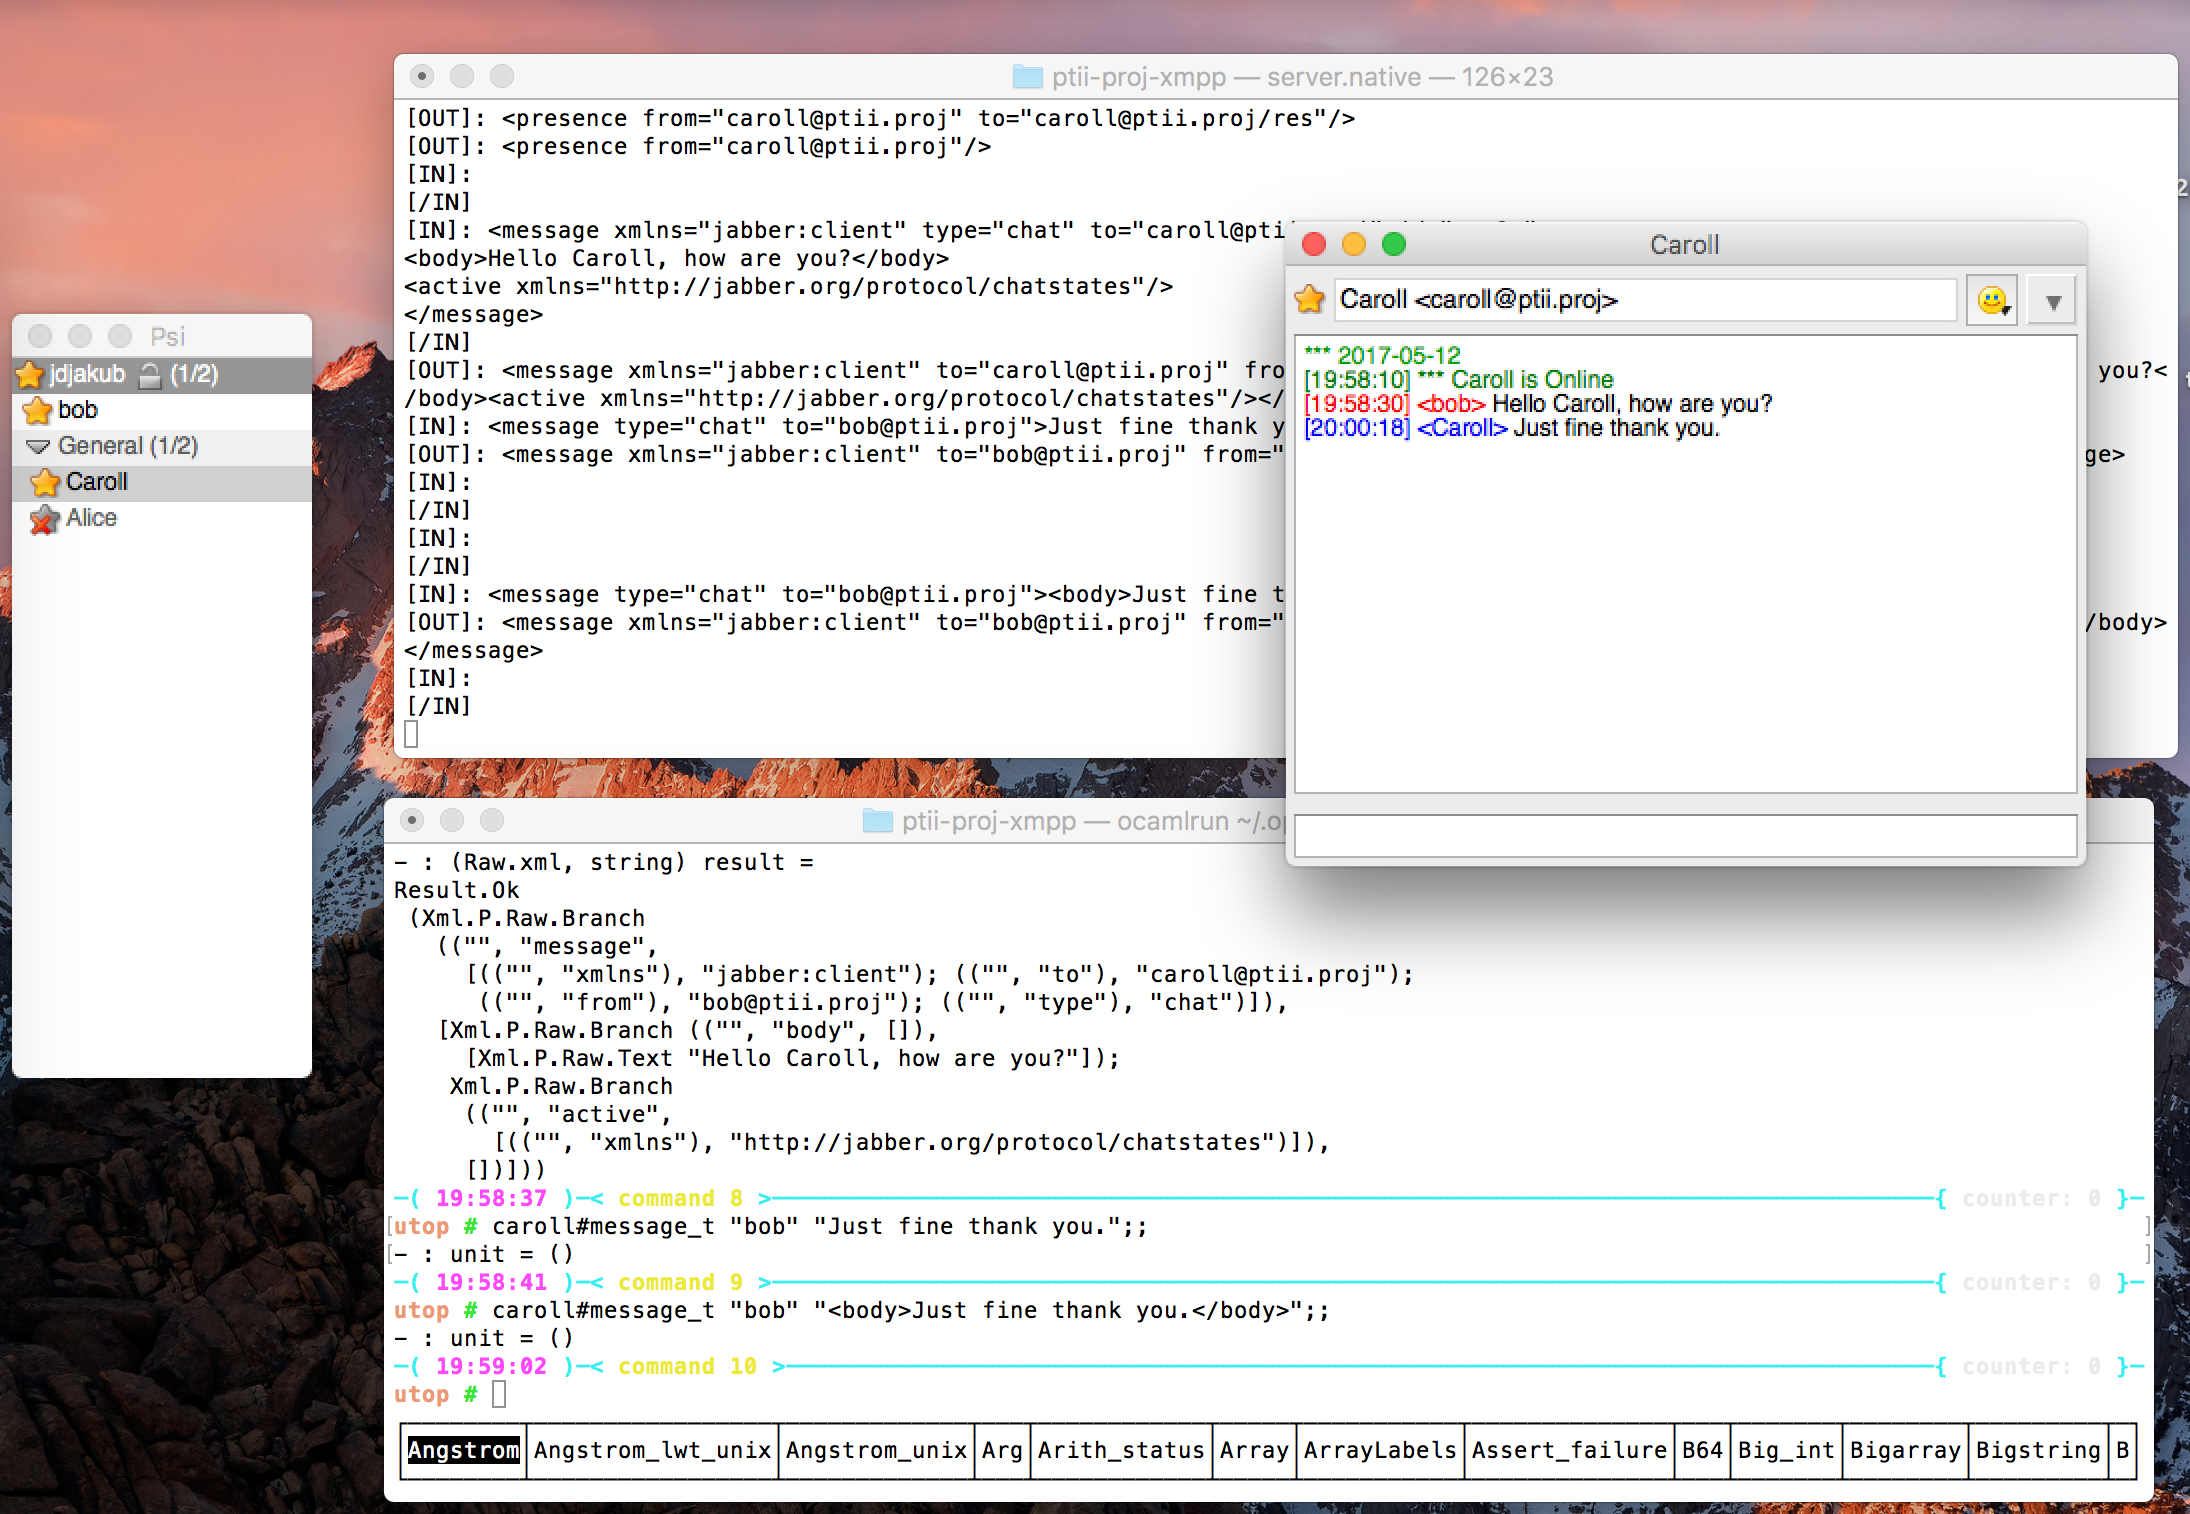
\includegraphics[width=\textwidth]{../transcripts/caroll_msg.png}
  \caption{Conversation between Bob (Psi) and Caroll (\code{Client} module).}
  \label{fig:caroll-msg}
\end{figure}

\section{Messaging}
\subsection{Throughput}
My primary aim was to see how throughput of message delivery was affected by the number of connected clients. To do this, I somehow needed a throughput figure for different client counts. Thus, I investigated how throughput varied over time for different client counts, hoping to see the value stabilise.

To keep the client controller simple, I adopted following model: $n$ clients send a fixed message to $n$ other clients, as fast as possible, until the program is manually terminated. To begin with, I used a 445-byte text string which, when wrapped in the XML \code{message} element, ran over the 512-byte size of the parsing buffers. This meant the figures would incorporate the buffering behaviour of the server and complete the worst-case behaviour under constant requests from clients.

The server samples its throughput at regular intervals and outputs the values. It does this by keeping track of how many messages it delivered in the last 5 seconds; this message count is then divided by the actual time elapsed, which stays close to 5 seconds.

\section{Procedure}
I began by observing the time-throughput curve for $n=20$, 40, and 60. For $n=70$ and above, the server demonstrated its breaking point by causing itself and the other applications on my computer to hang and require a forced reboot. I stopped there and started filling in the gaps between the other values; unfortunately, time did not premit further investigation of this issue.

As I ran the server five times for each value of $n$, I noticed that the performance of each repeat tended to be lower than those before it, and became more chaotic the longer it ran. This was unexpected; each test was done on a fresh, restarted instance of the server binary.

I hypothesised that these effects were due to the heating effect of the tests on my MacBook, which does not have a fan; to cool down, the CPU is throttled, necessarily reducing performance. I was performing the test runs in quick succession, one after the other, hence only the first instance would not suffer from prior heating.

To see if this was the case, I considered the most wildly fluctuating of the graphs, $n=20$, and repeated the five runs, this time allowing my machine to cool before each. The results (Figure~\ref{fig:20hotcold}) stood in stark contrast to the `hot' runs, with much less variation among the curves and a largely reduced downward trend.

I then ran hot/cold tests for $n=5$ with a very small message size, to give the server every opportunity for peak performance. These results were similar (Figure~\ref{fig:5hotcold}), and I made sure to perform the main throughput tests with cooling-off periods.

\begin{figure}
  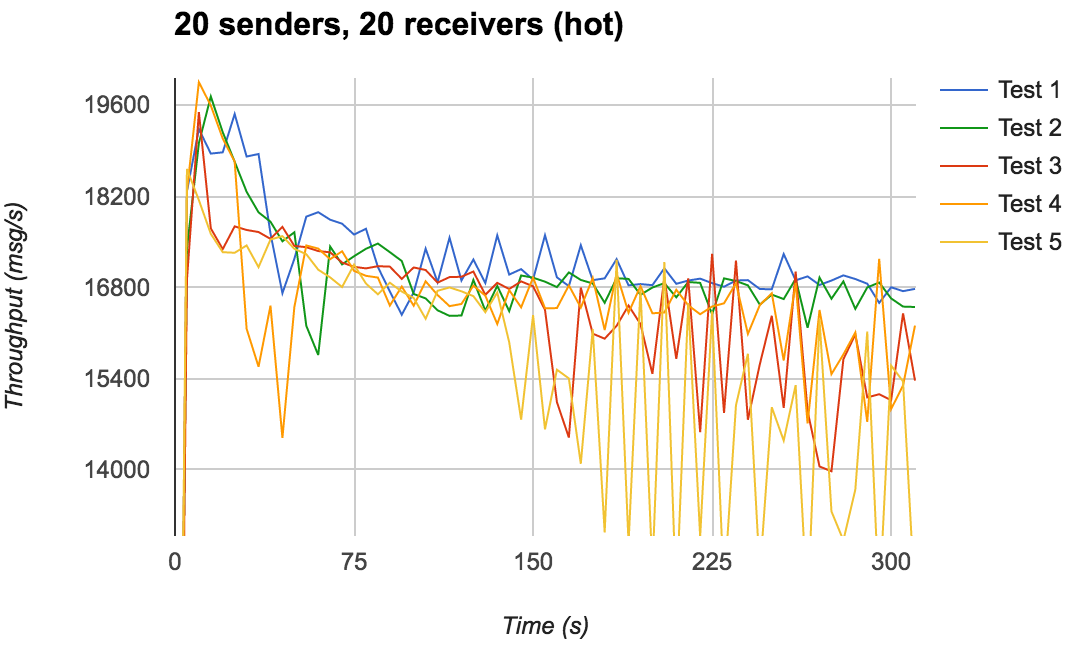
\includegraphics[width=0.5\textwidth]{../transcripts/lipsum/20n20/hot/hot.png}
  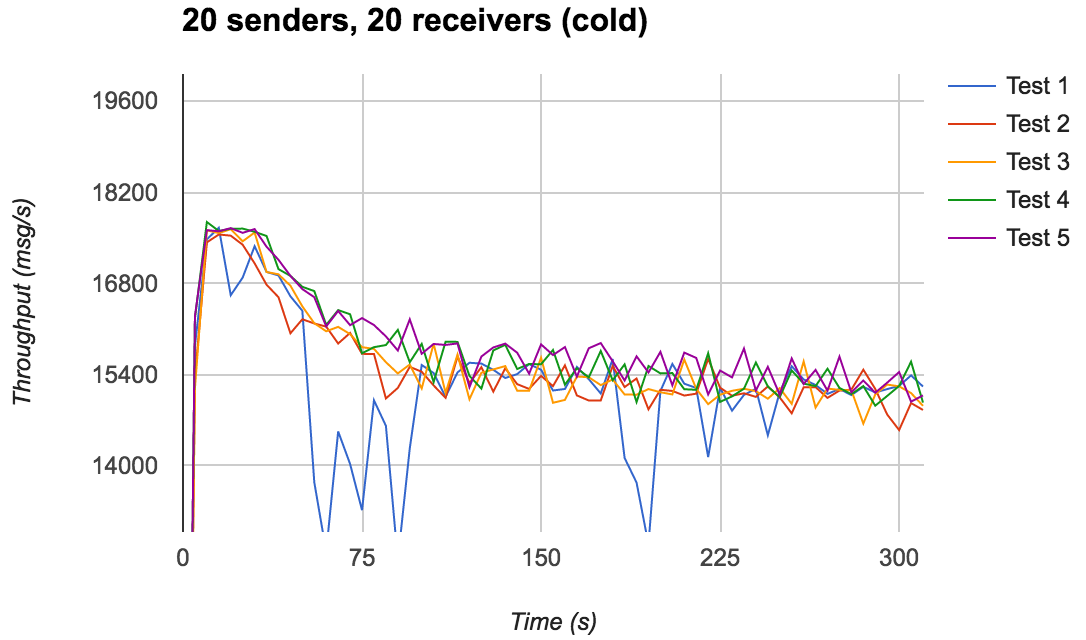
\includegraphics[width=0.5\textwidth]{../transcripts/lipsum/20n20/cold/cold.png}
  \caption{Effect of heating on throughput behaviour.}
  \label{fig:20hotcold}
\end{figure}

\begin{figure}
  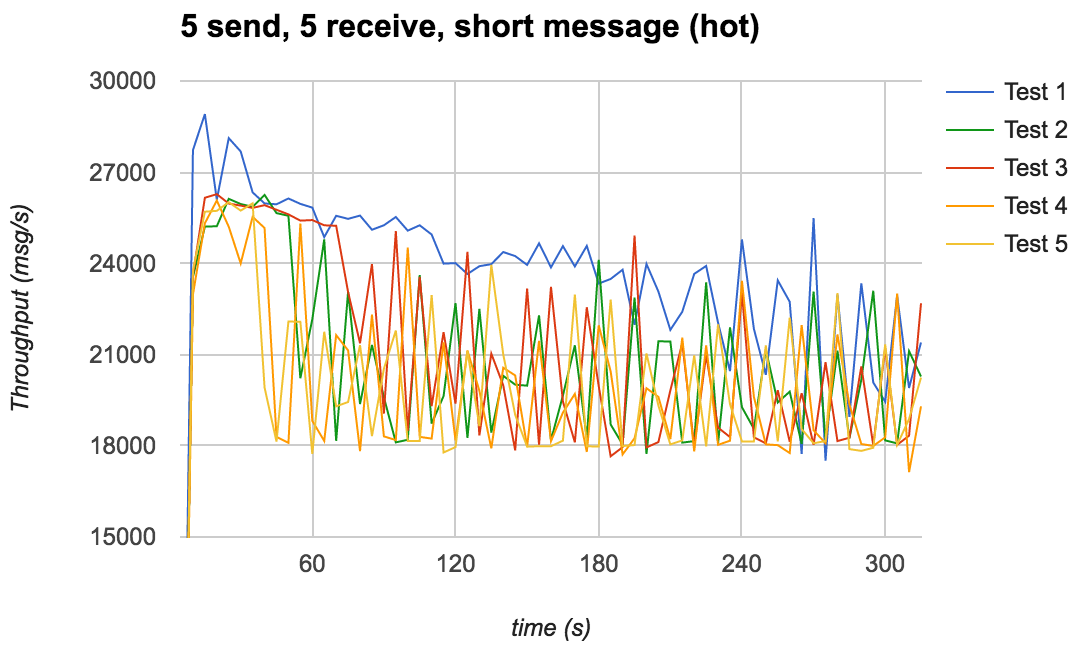
\includegraphics[width=0.5\textwidth]{../transcripts/hi/5n5/hot/hot.png}
  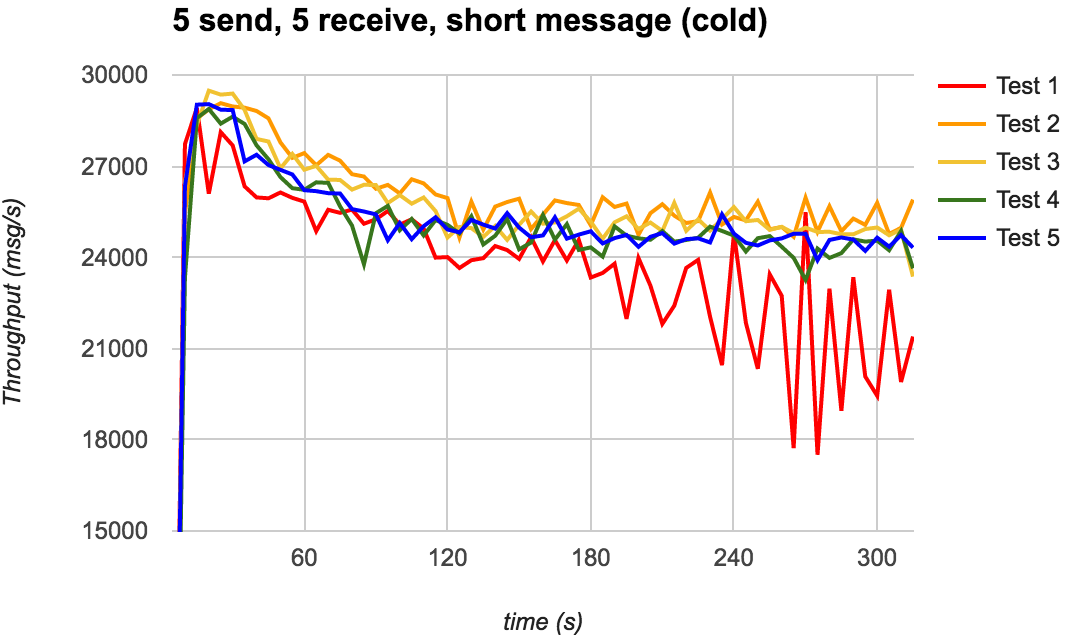
\includegraphics[width=0.5\textwidth]{../transcripts/hi/5n5/cold/cold.png}
  \caption{Further demonstration of the heating effect.}
  \label{fig:5hotcold}
\end{figure}

\subsubsection{Results and comments}
I obtained time-throughput characteristics for $n=5$, 10, 20, 30, 40 and 60. Overall, they remained reasonably stable after $t=100s$, after an initial transient with higher peak value.

Figure~\ref{fig:example-chstic} is an example of this. The steep rise at the beginning is an artefact caused by an initial throughput sample of $0$ just before the effect of the clients is felt, and can be ignored. The decay from an initial peak is likely due to the filling of the buffers in the OS kernel, which are much larger than my server's 512-byte buffers. The different repeats all stabilise fairly close to one another. The rest of the graphs share these patterns --- see Appendix~\ref{apdx:graphs} for details.

\begin{figure}
  \centering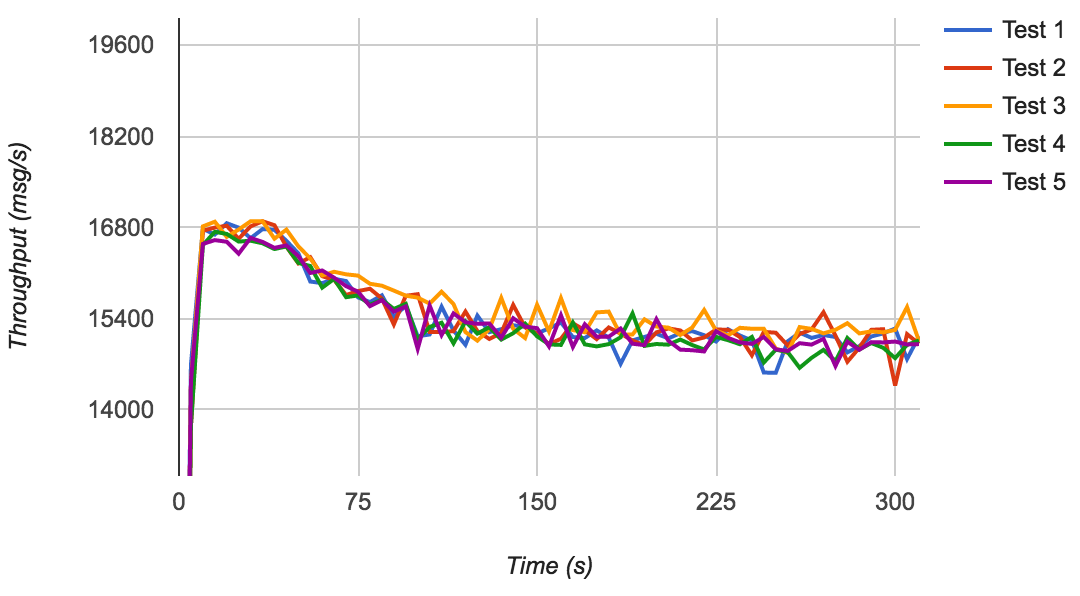
\includegraphics[width=\textwidth]{../transcripts/lipsum/30n30/cold.png}
  \caption{Graph of the 5 repeats performed for $n=30$, showing decay from peak and gradual stabilisation.}
  \label{fig:example-chstic}
\end{figure}

As the number $n$ of client pairs increases, the general trend is for the throughput to decrease. To display this visually on a 2-D plot, I obtained a set of values for each $n$. I took the minimum, maximum, median and lower/upper-quartile values of each repeat, and averaged them across the repeats. The resulting values were incorporated as the box-plots in Figure~\ref{fig:summary}.

\begin{figure}
  \centering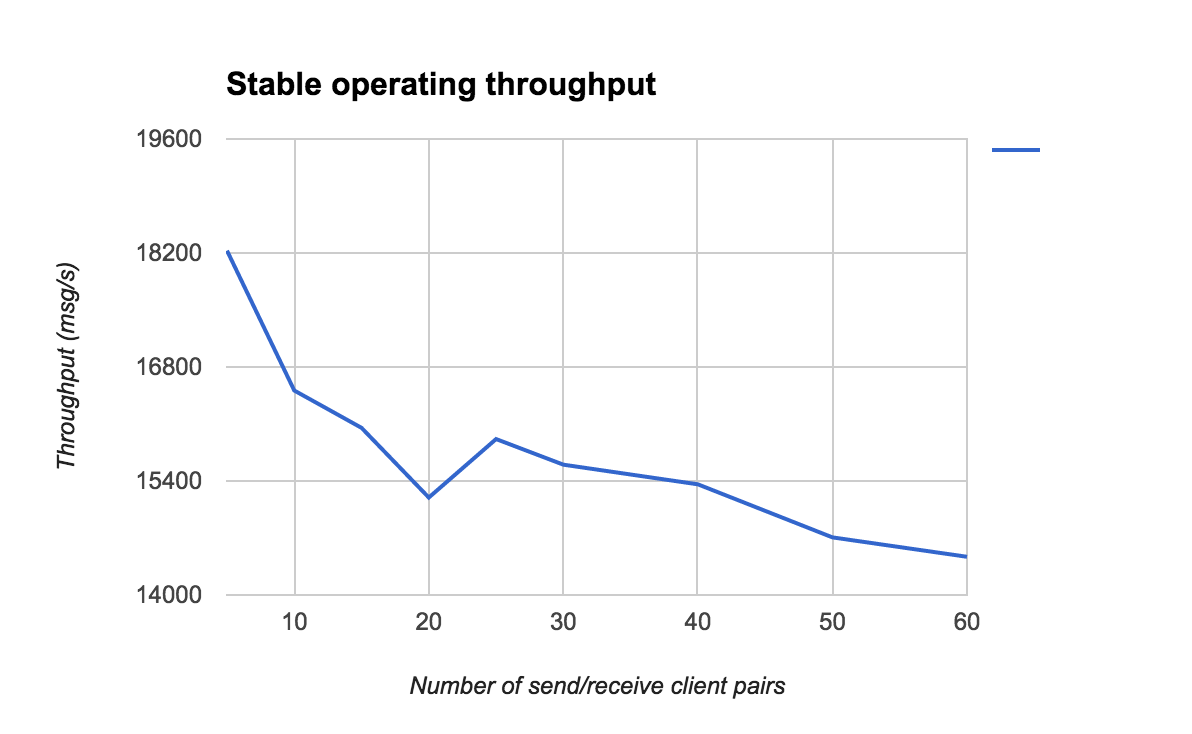
\includegraphics[width=\textwidth]{../transcripts/lipsum/throughp_clients.png}
  \caption{Effect of client load on operating throughput.}
  \label{fig:summary}
\end{figure}
